\documentclass{beamer}

\usepackage[polish]{babel}
\usepackage[Cp1250]{inputenc}
\usepackage[OT4]{fontenc}
\usepackage{beamerthemeshadow}
\usepackage{fancyvrb}
\usepackage{graphicx}
\usepackage{url}

\beamertemplateballitem
\beamertemplatenumberedballsectiontoc
\setbeamertemplate{footline}[frame number]
\setbeamertemplate{navigation symbols}{}

%\setbeamertemplate{background canvas}[vertical shading][top=blue!10,bottom=white]
\newtheorem{elements}[theorem]{Elementy}
\newtheorem{idatabase}[theorem]{Indukcyjna baza danych}
\hypersetup{%
  pdftitle={Salomon},%
  pdfauthor={Nikodem Jura},
  pdfauthor={Krzysztof Rajda},
  pdfauthor={Marek Kisiel-Dorohinicki},
  pdfauthor={Bart�omiej �nie�y�ski}
  }

\title[TP-SI: Salomon]{\small{Salomon � komponentowa architektura indukcyjnej bazy danych\\
jako platformy uczenia maszynowego}}

\author{Nikodem Jura, Krzysztof Rajda,\\ Marek Kisiel-Dorohinicki, Bart�omiej �nie�y�ski}

\institute{
  AGH -- Katedra Informatyki}\date{\today}

\newcounter{minisection}
\newcommand{\minisectionframe}[1]{
\frame{
	\begin{center}
	#1
	\end{center}
}}

\newcommand{\smallhref}[1]{{\footnotesize\href{#1}{\url{#1}}}}

\begin{document}

\frame{\titlepage}

\section{Agenda}

\frame{
	\frametitle{Agenda}
	\begin{itemize}
		\item Wprowadzenie
		\item Prace pokrewne
		\item Koncepcja platformy Salomon
		\item Architektura systemu
		\item Przyk�adowe zastosowanie
		\item Kierunki rozwoju
	\end{itemize}
}

\section{Wprowadzenie}
%\subsection{Machine learning}
%\subsection{Indukcyjne bazy danych}
%\subsection{Zastosowania}

Integracja technologii baz danych z nowoczesnymi metodami indukcyjnego
generowania wiedzy wydaje si� dawa� istotne korzy�ci w perspektywie
budowy system�w wspomaganie decyzji. Systemy nazywane czasem
indukcyjnymi bazami danych potrafi� odpowiedzie� nie tylko na pytania,
dla kt�rych odpowied� znajduje si� w bazie danych, ale r�wnie� na
pytania, kt�re wymagaj� zsyntetyzowania i zastosowania wiarygodnej
wiedzy, wygenerowanej przez indukcyjne wnioskowanie z fakt�w z bazy
danych i wcze�niejszej wiedzy.  Indukcyjne bazy danych mog� by�
postrzegane jako naturalny krok w rozwoju system�w bazodanowych \cite{bib3}.

\begin{figure}[ht]
    \centering
        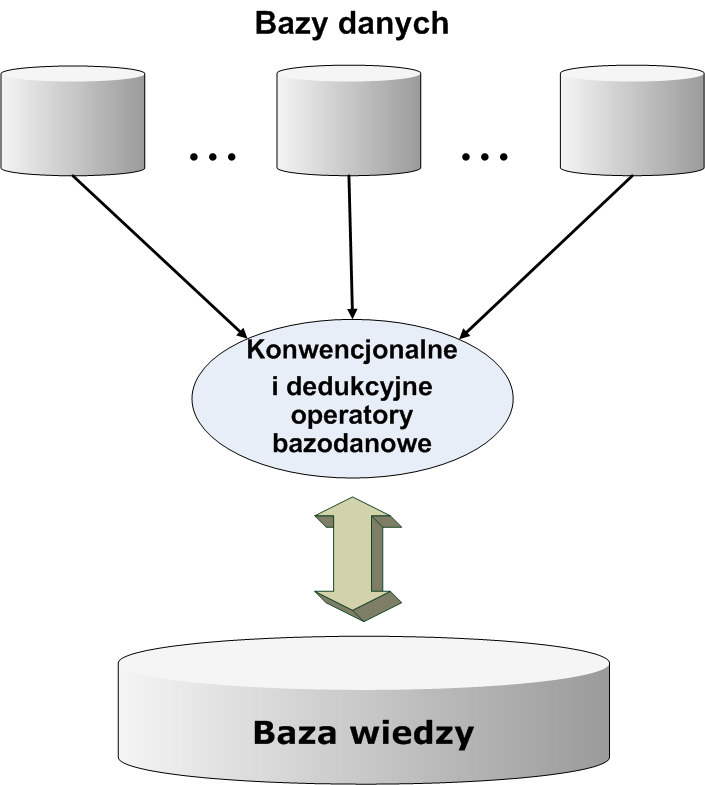
\includegraphics[width=0.70\textwidth]{img/knowledge_mining.png}
    \caption{Indukcyjne bazdy danych}
    \label{fig:architecture}
\end{figure}

\bigskip
W pracy przedstawiona zostanie architektura i wybrane aspekty
implementacji platformy \emph{Salomon}, jak r�wnie� zaprezentowane
zostan� mo�liwo�ci jego wykorzystania na przyk�adzie wybranych
algorytm�w pozyskiwania wiedzy z danych.

%\newpage
\section{Prace pokrewne}

\frame{
	\frametitle{Prace pokrewne}
	\begin{itemize}
		\item Weka
			\begin{itemize}
				\item Narz�dzie do prowadzenia eksperyment�w zwi�zanych z~uczeniem maszynowym
				\item Implementuje wiele r�nych rodzaj�w algorytm�w
				\item Wykorzystywana w zastosowaniach akademickich
			\end{itemize}		
		\item YALE
			\begin{itemize}
				\item R�norodno�� operator�w -- klasyfikuj�ce, klastruj�ce, asocjacyjne, oparte o drzewa decyzyjne
				\item Mo�liwo�� tworzenia ,,�a�cuch�w'' z�o�onych z r�nych problem�w
			\end{itemize}		
		\item Vinlen		
			\begin{itemize}
				\item Prekursor system�w realizuj�cych koncepcj� indukcyjnej bazy danych
				\item Rozwijany na \emph{George Mason University} pod opiek� prof. Ryszarda Michalskiego
			\end{itemize}
	\end{itemize}	
}
\section{Za�o�enia i koncepcja platformy}

\frame{
	\frametitle{Analiza wymaga�}
	\begin{itemize}		
		\item Przyjazny interfejs u�ytkownika
		\item Dobrze zdefiniowany interfejs programistyczny
		\item Odizolowanie algorytm�w od szczeg��w implementacyjnych platformy
		\item Sp�jna reprezentacja wiedzy dla wszystkich algorytm�w
		\item Komponentowa architektura
		\item Wykorzystanie gotowych implementacji algorytm�w
		\item Otwarta licencja \emph{(LGPL)}
	\end{itemize}		
}

\frame{
	\frametitle{G��wne za�o�enia}
	\begin{itemize}
			\item Koncepcja zadaniowo�ci			
			\begin{itemize}
				\item Zadanie -- atomowa jednostka reprezentuj�ca obliczenia
				\item Tworzenie powi�za� mi�dzy zadaniami
			\end{itemize}
    	\item Budowa komponentowa
    	\item Otwarto�� architektury
    	\item Niezale�no�� od �rodowiska wdro�enia
    	\item Prostota u�ytkowania
    \end{itemize}
}


\section{Architektura}

%diagram

System zosta� podzielony na 3 g��wne cz�ci: platform�, kontrolery
i~pluginy.

\begin{figure}[htb]
	\centering
		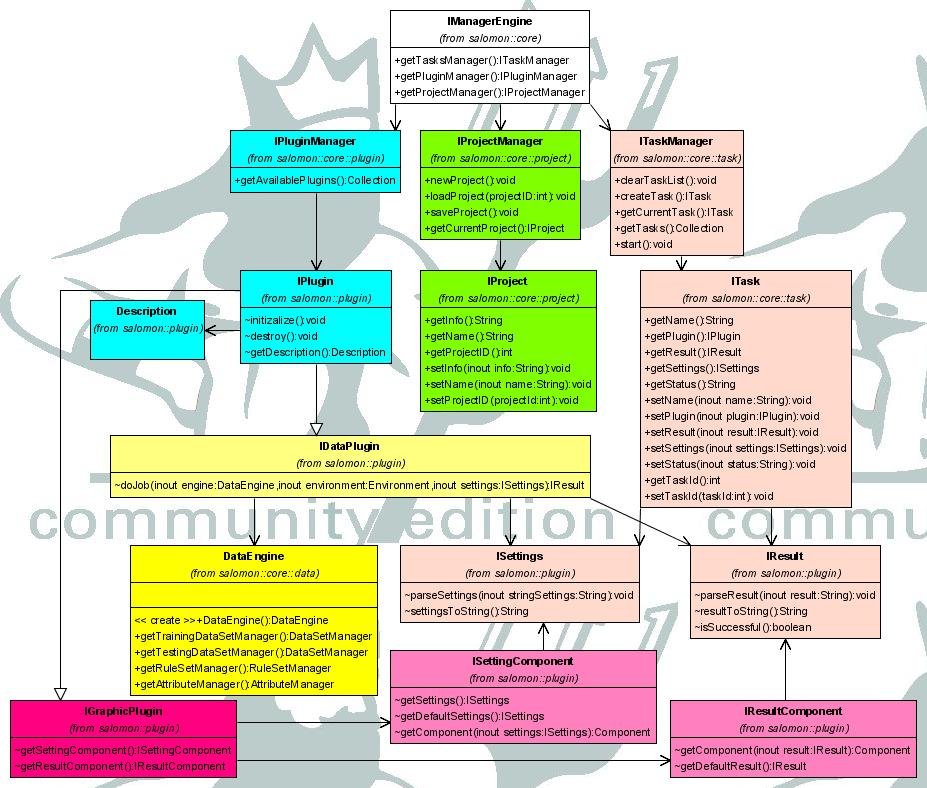
\includegraphics[width=0.90\textwidth]{img/uml/core.jpg}
	\caption{G��wne klasy systemu}
	\label{fig:core}
\end{figure}


\subsection{Platforma}

Dostarcza podstawowej funkcjonalno�ci  umo�liwiaj�cej prac� ca�ego
systemu,  �aduje odpowiedni kontroler, wczytuje pluginy, uruchamia
zadania. Za poszczeg�lne zadania odpowiadaj� odpowiednie menad�ery.

Menad�ery nie s� dost�pne bezpo�rednio z platformy, ale
przekazywane s� pluginom poprzez klas� \emph{DataEngine}. Dotyczy
to tylko klasy \emph{DataSetManager} i \emph{RuleSetManager},
pozosta�e nie s� dost�pne dla plugin�w. Plugin, zale�nie od
potrzeb, pobiera z niego potrzebny mu menad�er i za jego
po�rednictwem wykonuje operacje na bazie danych.

Bardzo wa�nym mechanizmem Salomona jest mo�liwo�� tworzenia powi�za� mi�dzy poszczeg�lnymi zadaniami. Wynik jednego zadania mo�e pos�u�y� jako wej�cie nast�pnego. Salomon w tym celu dostarcza �rodowisko. Wtyczka w trakcie wykonywania zadania opr�cz dost�pu  do manad�er�w posiada r�wnie� dost�p do �rodowiska, z kt�rego mo�e pobra� warto�ci zmiennych �rodowiskowych. Dane �rodowisko tworzone jest na pocz�tku wykonania listy zada� i przekazywane jest kolejno do nast�pnego zadania. Wtyczka w trakcie pracy mo�e modyfikowa� �rodowisko poprzez dodawanie, usuwanie oraz edycj� poszczeg�lnych zmiennych. W ten spos�b poszczeg�lne zadania mog� mi�dzy sob� przekazywa� informacje. Zmienne �rodowiskowe, podobnie jak ustawienia i rezultaty zada�, s� persystentne, a co za tym idzie potrzebny jest mechanizm serializacji i deserializacji.

W obecnej wersji mechanizm ten jest bardzo ubogi  - pozwala on na przekazywanie wy��cznie danych tekstowych. Wraz z pojawieniem si� kolejnej wersji, zmienne �rodowiskowe wykorzystywa� b�d� nowy mechanizm serializacji. Mo�liwo�� tworzenia zmiennych �rodowiskowych przez wtyczki mo�e rodzi� wiele problem�w z zapewnieniem kompatybilno�ci mi�dzy r�nymi wersjami wtyczek, komunikuj�cych si� ze sob�, dlatego te� aby unikn�� takich problem�w, ka�da wtyczka zmuszona b�dzie dostarczy� opis zmiennych, kt�re mo�e tworzy�.

W kolejnej wersji Salomona dodane zostan� klasy odpowiedzialne za przechowywanie danych. Klasy te b�d� odpowiada� poszczeg�lnym typom prostym oraz strukturze (struktura b�dzie mog�a zawiera� inne struktury oraz typy proste). Za pomoc� takich element�w, programista b�dzie m�g� stworzy� hierarchiczne struktury danych. Wprowadzenie takiego mechanizmu podyktowane jest potrzeb� ukrycia przed programist� sposobu zapisu danych w bazie lub w pliku. W obecnej wersji Salomona, tw�rca wtyczki musi dostarczy� mechanizm serializacji oraz deserializacji ustawie� i rezultat�w zada� do napisu � taki mechanizm niesie za sob� niebezpiecze�stwo niepoprawno�ci oraz nieefektywno�ci implementacji. Dostarczenie sp�jnego modelu seralizacji danych pozwala na niewidoczny dla wtyczek spos�b podmiany implementacji na bardziej efektywn� itp. Mechanizm ten mo�e okaza� si� r�wnie� po�yteczny po dodaniu do Salomona mo�liwo�ci definiowania zada� w pliku (np. XML). Seralizacja danych mo�e odbywa� si� do wielu format�w np. XML, CSV, tabel w bazie danych itp. 


\newpage

\subsection{DataEngine}
Klasa przekazywana pluginom podczas ich wykonania.
Za pomoc� pobieranych z niej menad�er�w (\emph{DataSetManager}, \emph{RuleSetManager}, w przysz�o�ci \emph{AttributeManager} i inne) wtyczki mog� operowa� na danych znajduj�cych si� w bazie.

\begin{figure}[htb]
	\centering
		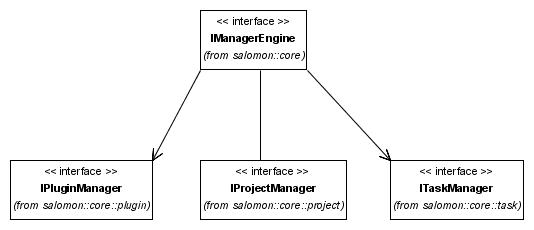
\includegraphics[width=0.80\textwidth]{img/uml/manager_engine.jpg}
	\caption{Interfejsy do zarz�dzania wiedz�}
	\label{fig:manager_engine}
\end{figure}

\subsubsection{DBManager}
Odpowiada za po��czenie z baz� danych. Dostarcza metody
zapewniaj�ce dost�p do danych przechowywanych w bazie. Swoj�
funkcjonalno�� udost�pnia odpowiednim menad�erom.

\subsubsection{DataSetManager}
Zarz�dza zbiorami danych. Pozwala tworzy� nowe podzbiory danych na
podstawie zawartych w bazie informacji oraz umo�liwia operowanie
na nich.
\subsubsection{RuleSetManager}
Zarz�dza regu�ami. Pozwala tworzy� nowe regu�y oraz
zarz�dza dost�pem do ju� istniej�cych.

\newpage

\subsubsection{IManagerEngine}
Klasa zarz�dza pozosta�ymi menad�erami. Utrzymuje jedn� instancj� ka�dego z nich 
i udost�pnia je pozosta�ym klasom z platformy.

\begin{figure}[htb]
	\centering
		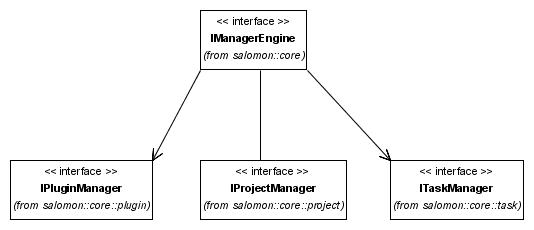
\includegraphics[width=0.90\textwidth]{img/uml/manager_engine.jpg}
	\caption{G��wna klasa zarz�dzaj�ca}
	\label{fig:manager_engine}
\end{figure}

\subsubsection{IProjectManager}
Zarz�dza projektami. Pozwala na utworzenie nowego
projektu, zapisanie bie��cego do bazy danych oraz na za�adowanie z bazy.

\subsubsection{IPluginManger}
Zarz�dza pluginami. Pozwala na utworzenie zapisanie informacji o nowym pluginie (jego nazwa, lokalizacja) oraz na pobranie listy dost�pnych plugin�w.

\subsubsection{ITaskManger}
Zarz�dza zadaniami. 

\subsection{Kontrolery}
Kontrolery odpowiadaj� za interakcj�
systemu z otoczeniem. W zale�no�ci od konfiguracji systemu przy
starcie uruchamiany jest jeden z kontroler�w. Kontrolery operuj�
na danych poprzez wsp�lny interfejs, a co za tym idzie, dane
utworzone poprzez jeden z nich s� dost�pne pomi�dzy kolejnymi
uruchomieniami programu dla pozosta�ych kontroler�w.

\subsubsection{LocalController}
Jest najprostszym kontrolerem. Zarz�dza zadaniami wykonywanymi na lokalnym komputerze. S� one
wykonywane sekwencyjnie. Zadaniem tego kontrolera jest dostarczenie
interfejsu u�ytkownika, pozwalaj�cego na zarz�dzanie projektami,
wtyczkami i zadaniami.

\subsubsection{MasterController}
Zadaniem tego kontrolera jest dostarczenie interfejsu do
zarz�dzania zdalnymi kontrolerami (\emph{ServantController}). Po
uruchomieniu nas�uchuje na po��czenia od klient�w, rozdziela
zadania oraz wy�wietla ich wyniki.

\subsubsection{ServantController}
Zadaniem tego kontrolera jest odszukanie g��wnego kontrolera
(\emph{MasterController}), zarejestrowanie si� i udost�pnianie mu
swoich us�ug. Ta wersja kontrolera nie posiada GUI, zarz�dzanie
nim odbywa si� za pomoc� klasy \emph{MasterController}.


\subsection{Pluginy}
G��wna funkcjonalno�� zosta�a  przeniesiona
do plugin�w, zadaniem systemu jest tylko zarz�dzanie ich
wykonaniem. Dzi�ki takiemu podej�ciu system jest �atwo skalowalny
i rozszerzalny o nowe mo�liwo�ci. Ka�dy z plugin�w musi
implementowa� nast�puj�ce interfejsy:


\subsubsection{IGraphicPlugin}
Pozwala pobra� parametry od u�ytkownika, kt�re nast�pnie zostan�
przekazane do plugin�w  przed ich wykonaniem. Zawiera dwie metody:
\emph{getSettingsPanel()}  i \emph{getResultPanel()}.  Pierwsza z
metod zwraca panel s�u��cy do konfiguracji pluginu, druga � panel,
na kt�rym prezentowane s� wyniki jego dzia�ania.

\subsubsection{IDataPlugin}
Posiada tylko jedn� metod� \emph{doJob()}. Przyjmuje ona jako
parametry obiekt klasy \emph{Environment}, reprezentuj�cy aktualny
stan systemu; \emph{DataEngine}, kt�ry umo�liwia operowanie na
bazie danych i \emph{ISettings}, reprezentuj�cy ustawienia
pluginu. Zwracany jest obiekt klasy \emph{IResult}, stanowi�cy
rezultat wykonania zadania.
\section{Przyk�adowe zastosowanie}

W ramach zaj�� na uczelni, zosta�a podj�ta pr�ba zaimplementowania 
algorytm�w drzew decyzyjnych w oparciu o platform� \emph{Salomon}.

Zgodnie z architektur� systemu, problem zaimplementowany zosta� 
za pomoc� odpowiednich wtyczek, z kt�rych ka�da przeznaczona by�a 
do realizacji osobnego etapu oblicze�.

Zadaniem pierwszej z nich jest konfiguracja procesu przetwarzania 
danych. Pozwala ona na wyb�r cechy, wzgl�dem kt�rej tworzone jest 
drzewo decyzyjne oraz cech, kt�re s� brane pod uwag� przy jego budowie.
Wyb�r ten odbywa si� przy u�yciu graficznego interfejsu u�ytkownika 
i mo�e dotyczy� dowolnej tematyki, zale�nie od danych, na kt�rych 
maj� by� przeprowadzane obliczenia. 
W naszym przypadku na podstawie kilku cech opisuj�cych kandydat�w do pracy, 
takich jak np. wiek, do�wiadczenie zawodowe, znajomo�� j�zyk�w obcych, 
tworzone by�o drzewo maj�ce na celu da� odpowied� na pytanie, 
czy dany kandydat powinien by� zatrudniony.

Druga wtyczka jest w�a�ciw� wtyczk� obliczeniow� -- jej zadaniem jest 
dostarczenie algorytmu, za pomoc� kt�rego tworzone jest drzewo. 
Dla cel�w demonstracyjnych wybrany zosta� jeden 
z najprostszych algorytm�w -- ID3.

Ostatnia wtyczka ma na celu wizualizacj� utworzonego przez 
wtyczk� algorytmiczn� drzewa w celu przedstawienia jej u�ytkownikowi.
W~obecnej wersji drzewo to przedstawiane jest w formie tekstowej, 
jednak�e dzi�ki niezale�no�ci poszczeg�lnych wtyczek od siebie, 
nic nie stoi na przeszkodzie, �eby doda� stworzy� now�, 
kt�ra realizuje wizualizacj� w dowolny inny spos�b.


\section{Podsumowanie}
%\subsection{Aktualny stan prac}
\emph{Salomon} nadal znajduje si� w bardzo wczesnym etapie rozwoju.
Nie mo�e by� wykorzystywany w �rodowisku produkcyjnym. Jednak ju� na obecnym poziomie
wykorzystanie \emph{Salomona} do tworzenia drzew decyzyjnych zosta�o zako�czone sukcesem.
To przyk�adowe zastosowanie pozwoli�o udowodni�, �e zaproponowana architektura z powodzeniem,
mo�e by� zastosowana w tego typu zagadnieniach.

\subsection{Przysz�e prace}
Do g��wnych zada� na przysz�o�� nale��:
\begin{itemize}
	\item Dodanie wsparcia dla mechanizmu skaut�w. \\
	
	Obecnie w systemie mo�e zosta� odpalona pojedynczy zestaw zada� jednocze�nie.
	Lista tych zada� zostanie zamieniona grafowym modelem przep�ywu wiedzy i danych
	i mo�liwe b�dzie definiowanie wielu na raz dzia�aj�cych graf�w zada�, kt�re b�d� reagowa�
	na zdarzenia, takie jak, przyk�adowo, pojawienie si� nowych danych w zewn�trznej bazie danych.
	
	\item Wsparcia dla innych typ�w wiedzy poza drzewami. \\
	
	W nast�pnej kolejno�ci, chcieliby�my doda� wsparcie dla regu�.
	
	\item Rozszerzenie wykorzystania rozproszonej architektury.
	
	Poszczeg�lne instancje komunikuj� si� ze sob�, jednak�e brakuje mechanizmu zapewniaj�cego
	najbardziej optymalne rozdzielenie zada�.
	
	\item Dodanie wsparcia dla innych �r�de� danych (wsparcie dla bazy \emph{Firebird}, r�wnie� nie jest kompletne)
\end{itemize}


%\subsection{Przysz�e prace}
%\subsection{Ewentualne zastosowania}
%Do najwa�niejszych przysz�ych pot�cialnych zastosowana� nale�y zaliczy� pomo
%\begin{itemize}
%	\item co zrobiono
%	\item zalety
%	\item braki
%	\item przyszle prace
%	\item ewentualne zastosowania
%\end{itemize}

\frame{
	\begin{center}
		 \LARGE{Dzi�kujemy za uwag�!}
	\end{center}
}

\end{document}
